\documentclass[11pt]{article}

    \usepackage[breakable]{tcolorbox}
    \usepackage{parskip} % Stop auto-indenting (to mimic markdown behaviour)
    

    % Basic figure setup, for now with no caption control since it's done
    % automatically by Pandoc (which extracts ![](path) syntax from Markdown).
    \usepackage{graphicx}
    % Keep aspect ratio if custom image width or height is specified
    \setkeys{Gin}{keepaspectratio}
    % Maintain compatibility with old templates. Remove in nbconvert 6.0
    \let\Oldincludegraphics\includegraphics
    % Ensure that by default, figures have no caption (until we provide a
    % proper Figure object with a Caption API and a way to capture that
    % in the conversion process - todo).
    \usepackage{caption}
    \DeclareCaptionFormat{nocaption}{}
    \captionsetup{format=nocaption,aboveskip=0pt,belowskip=0pt}

    \usepackage{float}
    \floatplacement{figure}{H} % forces figures to be placed at the correct location
    \usepackage{xcolor} % Allow colors to be defined
    \usepackage{enumerate} % Needed for markdown enumerations to work
    \usepackage{geometry} % Used to adjust the document margins
    \usepackage{amsmath} % Equations
    \usepackage{amssymb} % Equations
    \usepackage{textcomp} % defines textquotesingle
    % Hack from http://tex.stackexchange.com/a/47451/13684:
    \AtBeginDocument{%
        \def\PYZsq{\textquotesingle}% Upright quotes in Pygmentized code
    }
    \usepackage{upquote} % Upright quotes for verbatim code
    \usepackage{eurosym} % defines \euro

    \usepackage{iftex}
    \ifPDFTeX
        \usepackage[T1]{fontenc}
        \IfFileExists{alphabeta.sty}{
              \usepackage{alphabeta}
          }{
              \usepackage[mathletters]{ucs}
              \usepackage[utf8x]{inputenc}
          }
    \else
        \usepackage{fontspec}
        \usepackage{unicode-math}
    \fi

    \usepackage{fancyvrb} % verbatim replacement that allows latex
    \usepackage{grffile} % extends the file name processing of package graphics
                         % to support a larger range
    \makeatletter % fix for old versions of grffile with XeLaTeX
    \@ifpackagelater{grffile}{2019/11/01}
    {
      % Do nothing on new versions
    }
    {
      \def\Gread@@xetex#1{%
        \IfFileExists{"\Gin@base".bb}%
        {\Gread@eps{\Gin@base.bb}}%
        {\Gread@@xetex@aux#1}%
      }
    }
    \makeatother
    \usepackage[Export]{adjustbox} % Used to constrain images to a maximum size
    \adjustboxset{max size={0.9\linewidth}{0.9\paperheight}}

    % The hyperref package gives us a pdf with properly built
    % internal navigation ('pdf bookmarks' for the table of contents,
    % internal cross-reference links, web links for URLs, etc.)
    \usepackage{hyperref}
    % The default LaTeX title has an obnoxious amount of whitespace. By default,
    % titling removes some of it. It also provides customization options.
    \usepackage{titling}
    \usepackage{longtable} % longtable support required by pandoc >1.10
    \usepackage{booktabs}  % table support for pandoc > 1.12.2
    \usepackage{array}     % table support for pandoc >= 2.11.3
    \usepackage{calc}      % table minipage width calculation for pandoc >= 2.11.1
    \usepackage[inline]{enumitem} % IRkernel/repr support (it uses the enumerate* environment)
    \usepackage[normalem]{ulem} % ulem is needed to support strikethroughs (\sout)
                                % normalem makes italics be italics, not underlines
    \usepackage{soul}      % strikethrough (\st) support for pandoc >= 3.0.0
    \usepackage{mathrsfs}
    

    
    % Colors for the hyperref package
    \definecolor{urlcolor}{rgb}{0,.145,.698}
    \definecolor{linkcolor}{rgb}{.71,0.21,0.01}
    \definecolor{citecolor}{rgb}{.12,.54,.11}

    % ANSI colors
    \definecolor{ansi-black}{HTML}{3E424D}
    \definecolor{ansi-black-intense}{HTML}{282C36}
    \definecolor{ansi-red}{HTML}{E75C58}
    \definecolor{ansi-red-intense}{HTML}{B22B31}
    \definecolor{ansi-green}{HTML}{00A250}
    \definecolor{ansi-green-intense}{HTML}{007427}
    \definecolor{ansi-yellow}{HTML}{DDB62B}
    \definecolor{ansi-yellow-intense}{HTML}{B27D12}
    \definecolor{ansi-blue}{HTML}{208FFB}
    \definecolor{ansi-blue-intense}{HTML}{0065CA}
    \definecolor{ansi-magenta}{HTML}{D160C4}
    \definecolor{ansi-magenta-intense}{HTML}{A03196}
    \definecolor{ansi-cyan}{HTML}{60C6C8}
    \definecolor{ansi-cyan-intense}{HTML}{258F8F}
    \definecolor{ansi-white}{HTML}{C5C1B4}
    \definecolor{ansi-white-intense}{HTML}{A1A6B2}
    \definecolor{ansi-default-inverse-fg}{HTML}{FFFFFF}
    \definecolor{ansi-default-inverse-bg}{HTML}{000000}

    % common color for the border for error outputs.
    \definecolor{outerrorbackground}{HTML}{FFDFDF}

    % commands and environments needed by pandoc snippets
    % extracted from the output of `pandoc -s`
    \providecommand{\tightlist}{%
      \setlength{\itemsep}{0pt}\setlength{\parskip}{0pt}}
    \DefineVerbatimEnvironment{Highlighting}{Verbatim}{commandchars=\\\{\}}
    % Add ',fontsize=\small' for more characters per line
    \newenvironment{Shaded}{}{}
    \newcommand{\KeywordTok}[1]{\textcolor[rgb]{0.00,0.44,0.13}{\textbf{{#1}}}}
    \newcommand{\DataTypeTok}[1]{\textcolor[rgb]{0.56,0.13,0.00}{{#1}}}
    \newcommand{\DecValTok}[1]{\textcolor[rgb]{0.25,0.63,0.44}{{#1}}}
    \newcommand{\BaseNTok}[1]{\textcolor[rgb]{0.25,0.63,0.44}{{#1}}}
    \newcommand{\FloatTok}[1]{\textcolor[rgb]{0.25,0.63,0.44}{{#1}}}
    \newcommand{\CharTok}[1]{\textcolor[rgb]{0.25,0.44,0.63}{{#1}}}
    \newcommand{\StringTok}[1]{\textcolor[rgb]{0.25,0.44,0.63}{{#1}}}
    \newcommand{\CommentTok}[1]{\textcolor[rgb]{0.38,0.63,0.69}{\textit{{#1}}}}
    \newcommand{\OtherTok}[1]{\textcolor[rgb]{0.00,0.44,0.13}{{#1}}}
    \newcommand{\AlertTok}[1]{\textcolor[rgb]{1.00,0.00,0.00}{\textbf{{#1}}}}
    \newcommand{\FunctionTok}[1]{\textcolor[rgb]{0.02,0.16,0.49}{{#1}}}
    \newcommand{\RegionMarkerTok}[1]{{#1}}
    \newcommand{\ErrorTok}[1]{\textcolor[rgb]{1.00,0.00,0.00}{\textbf{{#1}}}}
    \newcommand{\NormalTok}[1]{{#1}}

    % Additional commands for more recent versions of Pandoc
    \newcommand{\ConstantTok}[1]{\textcolor[rgb]{0.53,0.00,0.00}{{#1}}}
    \newcommand{\SpecialCharTok}[1]{\textcolor[rgb]{0.25,0.44,0.63}{{#1}}}
    \newcommand{\VerbatimStringTok}[1]{\textcolor[rgb]{0.25,0.44,0.63}{{#1}}}
    \newcommand{\SpecialStringTok}[1]{\textcolor[rgb]{0.73,0.40,0.53}{{#1}}}
    \newcommand{\ImportTok}[1]{{#1}}
    \newcommand{\DocumentationTok}[1]{\textcolor[rgb]{0.73,0.13,0.13}{\textit{{#1}}}}
    \newcommand{\AnnotationTok}[1]{\textcolor[rgb]{0.38,0.63,0.69}{\textbf{\textit{{#1}}}}}
    \newcommand{\CommentVarTok}[1]{\textcolor[rgb]{0.38,0.63,0.69}{\textbf{\textit{{#1}}}}}
    \newcommand{\VariableTok}[1]{\textcolor[rgb]{0.10,0.09,0.49}{{#1}}}
    \newcommand{\ControlFlowTok}[1]{\textcolor[rgb]{0.00,0.44,0.13}{\textbf{{#1}}}}
    \newcommand{\OperatorTok}[1]{\textcolor[rgb]{0.40,0.40,0.40}{{#1}}}
    \newcommand{\BuiltInTok}[1]{{#1}}
    \newcommand{\ExtensionTok}[1]{{#1}}
    \newcommand{\PreprocessorTok}[1]{\textcolor[rgb]{0.74,0.48,0.00}{{#1}}}
    \newcommand{\AttributeTok}[1]{\textcolor[rgb]{0.49,0.56,0.16}{{#1}}}
    \newcommand{\InformationTok}[1]{\textcolor[rgb]{0.38,0.63,0.69}{\textbf{\textit{{#1}}}}}
    \newcommand{\WarningTok}[1]{\textcolor[rgb]{0.38,0.63,0.69}{\textbf{\textit{{#1}}}}}
    \makeatletter
    \newsavebox\pandoc@box
    \newcommand*\pandocbounded[1]{%
      \sbox\pandoc@box{#1}%
      % scaling factors for width and height
      \Gscale@div\@tempa\textheight{\dimexpr\ht\pandoc@box+\dp\pandoc@box\relax}%
      \Gscale@div\@tempb\linewidth{\wd\pandoc@box}%
      % select the smaller of both
      \ifdim\@tempb\p@<\@tempa\p@
        \let\@tempa\@tempb
      \fi
      % scaling accordingly (\@tempa < 1)
      \ifdim\@tempa\p@<\p@
        \scalebox{\@tempa}{\usebox\pandoc@box}%
      % scaling not needed, use as it is
      \else
        \usebox{\pandoc@box}%
      \fi
    }
    \makeatother

    % Define a nice break command that doesn't care if a line doesn't already
    % exist.
    \def\br{\hspace*{\fill} \\* }
    % Math Jax compatibility definitions
    \def\gt{>}
    \def\lt{<}
    \let\Oldtex\TeX
    \let\Oldlatex\LaTeX
    \renewcommand{\TeX}{\textrm{\Oldtex}}
    \renewcommand{\LaTeX}{\textrm{\Oldlatex}}
    % Document parameters
    % Document title
    \title{09\_notes}
    
    
    
    
    
    
    
% Pygments definitions
\makeatletter
\def\PY@reset{\let\PY@it=\relax \let\PY@bf=\relax%
    \let\PY@ul=\relax \let\PY@tc=\relax%
    \let\PY@bc=\relax \let\PY@ff=\relax}
\def\PY@tok#1{\csname PY@tok@#1\endcsname}
\def\PY@toks#1+{\ifx\relax#1\empty\else%
    \PY@tok{#1}\expandafter\PY@toks\fi}
\def\PY@do#1{\PY@bc{\PY@tc{\PY@ul{%
    \PY@it{\PY@bf{\PY@ff{#1}}}}}}}
\def\PY#1#2{\PY@reset\PY@toks#1+\relax+\PY@do{#2}}

\@namedef{PY@tok@w}{\def\PY@tc##1{\textcolor[rgb]{0.73,0.73,0.73}{##1}}}
\@namedef{PY@tok@c}{\let\PY@it=\textit\def\PY@tc##1{\textcolor[rgb]{0.24,0.48,0.48}{##1}}}
\@namedef{PY@tok@cp}{\def\PY@tc##1{\textcolor[rgb]{0.61,0.40,0.00}{##1}}}
\@namedef{PY@tok@k}{\let\PY@bf=\textbf\def\PY@tc##1{\textcolor[rgb]{0.00,0.50,0.00}{##1}}}
\@namedef{PY@tok@kp}{\def\PY@tc##1{\textcolor[rgb]{0.00,0.50,0.00}{##1}}}
\@namedef{PY@tok@kt}{\def\PY@tc##1{\textcolor[rgb]{0.69,0.00,0.25}{##1}}}
\@namedef{PY@tok@o}{\def\PY@tc##1{\textcolor[rgb]{0.40,0.40,0.40}{##1}}}
\@namedef{PY@tok@ow}{\let\PY@bf=\textbf\def\PY@tc##1{\textcolor[rgb]{0.67,0.13,1.00}{##1}}}
\@namedef{PY@tok@nb}{\def\PY@tc##1{\textcolor[rgb]{0.00,0.50,0.00}{##1}}}
\@namedef{PY@tok@nf}{\def\PY@tc##1{\textcolor[rgb]{0.00,0.00,1.00}{##1}}}
\@namedef{PY@tok@nc}{\let\PY@bf=\textbf\def\PY@tc##1{\textcolor[rgb]{0.00,0.00,1.00}{##1}}}
\@namedef{PY@tok@nn}{\let\PY@bf=\textbf\def\PY@tc##1{\textcolor[rgb]{0.00,0.00,1.00}{##1}}}
\@namedef{PY@tok@ne}{\let\PY@bf=\textbf\def\PY@tc##1{\textcolor[rgb]{0.80,0.25,0.22}{##1}}}
\@namedef{PY@tok@nv}{\def\PY@tc##1{\textcolor[rgb]{0.10,0.09,0.49}{##1}}}
\@namedef{PY@tok@no}{\def\PY@tc##1{\textcolor[rgb]{0.53,0.00,0.00}{##1}}}
\@namedef{PY@tok@nl}{\def\PY@tc##1{\textcolor[rgb]{0.46,0.46,0.00}{##1}}}
\@namedef{PY@tok@ni}{\let\PY@bf=\textbf\def\PY@tc##1{\textcolor[rgb]{0.44,0.44,0.44}{##1}}}
\@namedef{PY@tok@na}{\def\PY@tc##1{\textcolor[rgb]{0.41,0.47,0.13}{##1}}}
\@namedef{PY@tok@nt}{\let\PY@bf=\textbf\def\PY@tc##1{\textcolor[rgb]{0.00,0.50,0.00}{##1}}}
\@namedef{PY@tok@nd}{\def\PY@tc##1{\textcolor[rgb]{0.67,0.13,1.00}{##1}}}
\@namedef{PY@tok@s}{\def\PY@tc##1{\textcolor[rgb]{0.73,0.13,0.13}{##1}}}
\@namedef{PY@tok@sd}{\let\PY@it=\textit\def\PY@tc##1{\textcolor[rgb]{0.73,0.13,0.13}{##1}}}
\@namedef{PY@tok@si}{\let\PY@bf=\textbf\def\PY@tc##1{\textcolor[rgb]{0.64,0.35,0.47}{##1}}}
\@namedef{PY@tok@se}{\let\PY@bf=\textbf\def\PY@tc##1{\textcolor[rgb]{0.67,0.36,0.12}{##1}}}
\@namedef{PY@tok@sr}{\def\PY@tc##1{\textcolor[rgb]{0.64,0.35,0.47}{##1}}}
\@namedef{PY@tok@ss}{\def\PY@tc##1{\textcolor[rgb]{0.10,0.09,0.49}{##1}}}
\@namedef{PY@tok@sx}{\def\PY@tc##1{\textcolor[rgb]{0.00,0.50,0.00}{##1}}}
\@namedef{PY@tok@m}{\def\PY@tc##1{\textcolor[rgb]{0.40,0.40,0.40}{##1}}}
\@namedef{PY@tok@gh}{\let\PY@bf=\textbf\def\PY@tc##1{\textcolor[rgb]{0.00,0.00,0.50}{##1}}}
\@namedef{PY@tok@gu}{\let\PY@bf=\textbf\def\PY@tc##1{\textcolor[rgb]{0.50,0.00,0.50}{##1}}}
\@namedef{PY@tok@gd}{\def\PY@tc##1{\textcolor[rgb]{0.63,0.00,0.00}{##1}}}
\@namedef{PY@tok@gi}{\def\PY@tc##1{\textcolor[rgb]{0.00,0.52,0.00}{##1}}}
\@namedef{PY@tok@gr}{\def\PY@tc##1{\textcolor[rgb]{0.89,0.00,0.00}{##1}}}
\@namedef{PY@tok@ge}{\let\PY@it=\textit}
\@namedef{PY@tok@gs}{\let\PY@bf=\textbf}
\@namedef{PY@tok@ges}{\let\PY@bf=\textbf\let\PY@it=\textit}
\@namedef{PY@tok@gp}{\let\PY@bf=\textbf\def\PY@tc##1{\textcolor[rgb]{0.00,0.00,0.50}{##1}}}
\@namedef{PY@tok@go}{\def\PY@tc##1{\textcolor[rgb]{0.44,0.44,0.44}{##1}}}
\@namedef{PY@tok@gt}{\def\PY@tc##1{\textcolor[rgb]{0.00,0.27,0.87}{##1}}}
\@namedef{PY@tok@err}{\def\PY@bc##1{{\setlength{\fboxsep}{\string -\fboxrule}\fcolorbox[rgb]{1.00,0.00,0.00}{1,1,1}{\strut ##1}}}}
\@namedef{PY@tok@kc}{\let\PY@bf=\textbf\def\PY@tc##1{\textcolor[rgb]{0.00,0.50,0.00}{##1}}}
\@namedef{PY@tok@kd}{\let\PY@bf=\textbf\def\PY@tc##1{\textcolor[rgb]{0.00,0.50,0.00}{##1}}}
\@namedef{PY@tok@kn}{\let\PY@bf=\textbf\def\PY@tc##1{\textcolor[rgb]{0.00,0.50,0.00}{##1}}}
\@namedef{PY@tok@kr}{\let\PY@bf=\textbf\def\PY@tc##1{\textcolor[rgb]{0.00,0.50,0.00}{##1}}}
\@namedef{PY@tok@bp}{\def\PY@tc##1{\textcolor[rgb]{0.00,0.50,0.00}{##1}}}
\@namedef{PY@tok@fm}{\def\PY@tc##1{\textcolor[rgb]{0.00,0.00,1.00}{##1}}}
\@namedef{PY@tok@vc}{\def\PY@tc##1{\textcolor[rgb]{0.10,0.09,0.49}{##1}}}
\@namedef{PY@tok@vg}{\def\PY@tc##1{\textcolor[rgb]{0.10,0.09,0.49}{##1}}}
\@namedef{PY@tok@vi}{\def\PY@tc##1{\textcolor[rgb]{0.10,0.09,0.49}{##1}}}
\@namedef{PY@tok@vm}{\def\PY@tc##1{\textcolor[rgb]{0.10,0.09,0.49}{##1}}}
\@namedef{PY@tok@sa}{\def\PY@tc##1{\textcolor[rgb]{0.73,0.13,0.13}{##1}}}
\@namedef{PY@tok@sb}{\def\PY@tc##1{\textcolor[rgb]{0.73,0.13,0.13}{##1}}}
\@namedef{PY@tok@sc}{\def\PY@tc##1{\textcolor[rgb]{0.73,0.13,0.13}{##1}}}
\@namedef{PY@tok@dl}{\def\PY@tc##1{\textcolor[rgb]{0.73,0.13,0.13}{##1}}}
\@namedef{PY@tok@s2}{\def\PY@tc##1{\textcolor[rgb]{0.73,0.13,0.13}{##1}}}
\@namedef{PY@tok@sh}{\def\PY@tc##1{\textcolor[rgb]{0.73,0.13,0.13}{##1}}}
\@namedef{PY@tok@s1}{\def\PY@tc##1{\textcolor[rgb]{0.73,0.13,0.13}{##1}}}
\@namedef{PY@tok@mb}{\def\PY@tc##1{\textcolor[rgb]{0.40,0.40,0.40}{##1}}}
\@namedef{PY@tok@mf}{\def\PY@tc##1{\textcolor[rgb]{0.40,0.40,0.40}{##1}}}
\@namedef{PY@tok@mh}{\def\PY@tc##1{\textcolor[rgb]{0.40,0.40,0.40}{##1}}}
\@namedef{PY@tok@mi}{\def\PY@tc##1{\textcolor[rgb]{0.40,0.40,0.40}{##1}}}
\@namedef{PY@tok@il}{\def\PY@tc##1{\textcolor[rgb]{0.40,0.40,0.40}{##1}}}
\@namedef{PY@tok@mo}{\def\PY@tc##1{\textcolor[rgb]{0.40,0.40,0.40}{##1}}}
\@namedef{PY@tok@ch}{\let\PY@it=\textit\def\PY@tc##1{\textcolor[rgb]{0.24,0.48,0.48}{##1}}}
\@namedef{PY@tok@cm}{\let\PY@it=\textit\def\PY@tc##1{\textcolor[rgb]{0.24,0.48,0.48}{##1}}}
\@namedef{PY@tok@cpf}{\let\PY@it=\textit\def\PY@tc##1{\textcolor[rgb]{0.24,0.48,0.48}{##1}}}
\@namedef{PY@tok@c1}{\let\PY@it=\textit\def\PY@tc##1{\textcolor[rgb]{0.24,0.48,0.48}{##1}}}
\@namedef{PY@tok@cs}{\let\PY@it=\textit\def\PY@tc##1{\textcolor[rgb]{0.24,0.48,0.48}{##1}}}

\def\PYZbs{\char`\\}
\def\PYZus{\char`\_}
\def\PYZob{\char`\{}
\def\PYZcb{\char`\}}
\def\PYZca{\char`\^}
\def\PYZam{\char`\&}
\def\PYZlt{\char`\<}
\def\PYZgt{\char`\>}
\def\PYZsh{\char`\#}
\def\PYZpc{\char`\%}
\def\PYZdl{\char`\$}
\def\PYZhy{\char`\-}
\def\PYZsq{\char`\'}
\def\PYZdq{\char`\"}
\def\PYZti{\char`\~}
% for compatibility with earlier versions
\def\PYZat{@}
\def\PYZlb{[}
\def\PYZrb{]}
\makeatother


    % For linebreaks inside Verbatim environment from package fancyvrb.
    \makeatletter
        \newbox\Wrappedcontinuationbox
        \newbox\Wrappedvisiblespacebox
        \newcommand*\Wrappedvisiblespace {\textcolor{red}{\textvisiblespace}}
        \newcommand*\Wrappedcontinuationsymbol {\textcolor{red}{\llap{\tiny$\m@th\hookrightarrow$}}}
        \newcommand*\Wrappedcontinuationindent {3ex }
        \newcommand*\Wrappedafterbreak {\kern\Wrappedcontinuationindent\copy\Wrappedcontinuationbox}
        % Take advantage of the already applied Pygments mark-up to insert
        % potential linebreaks for TeX processing.
        %        {, <, #, %, $, ' and ": go to next line.
        %        _, }, ^, &, >, - and ~: stay at end of broken line.
        % Use of \textquotesingle for straight quote.
        \newcommand*\Wrappedbreaksatspecials {%
            \def\PYGZus{\discretionary{\char`\_}{\Wrappedafterbreak}{\char`\_}}%
            \def\PYGZob{\discretionary{}{\Wrappedafterbreak\char`\{}{\char`\{}}%
            \def\PYGZcb{\discretionary{\char`\}}{\Wrappedafterbreak}{\char`\}}}%
            \def\PYGZca{\discretionary{\char`\^}{\Wrappedafterbreak}{\char`\^}}%
            \def\PYGZam{\discretionary{\char`\&}{\Wrappedafterbreak}{\char`\&}}%
            \def\PYGZlt{\discretionary{}{\Wrappedafterbreak\char`\<}{\char`\<}}%
            \def\PYGZgt{\discretionary{\char`\>}{\Wrappedafterbreak}{\char`\>}}%
            \def\PYGZsh{\discretionary{}{\Wrappedafterbreak\char`\#}{\char`\#}}%
            \def\PYGZpc{\discretionary{}{\Wrappedafterbreak\char`\%}{\char`\%}}%
            \def\PYGZdl{\discretionary{}{\Wrappedafterbreak\char`\$}{\char`\$}}%
            \def\PYGZhy{\discretionary{\char`\-}{\Wrappedafterbreak}{\char`\-}}%
            \def\PYGZsq{\discretionary{}{\Wrappedafterbreak\textquotesingle}{\textquotesingle}}%
            \def\PYGZdq{\discretionary{}{\Wrappedafterbreak\char`\"}{\char`\"}}%
            \def\PYGZti{\discretionary{\char`\~}{\Wrappedafterbreak}{\char`\~}}%
        }
        % Some characters . , ; ? ! / are not pygmentized.
        % This macro makes them "active" and they will insert potential linebreaks
        \newcommand*\Wrappedbreaksatpunct {%
            \lccode`\~`\.\lowercase{\def~}{\discretionary{\hbox{\char`\.}}{\Wrappedafterbreak}{\hbox{\char`\.}}}%
            \lccode`\~`\,\lowercase{\def~}{\discretionary{\hbox{\char`\,}}{\Wrappedafterbreak}{\hbox{\char`\,}}}%
            \lccode`\~`\;\lowercase{\def~}{\discretionary{\hbox{\char`\;}}{\Wrappedafterbreak}{\hbox{\char`\;}}}%
            \lccode`\~`\:\lowercase{\def~}{\discretionary{\hbox{\char`\:}}{\Wrappedafterbreak}{\hbox{\char`\:}}}%
            \lccode`\~`\?\lowercase{\def~}{\discretionary{\hbox{\char`\?}}{\Wrappedafterbreak}{\hbox{\char`\?}}}%
            \lccode`\~`\!\lowercase{\def~}{\discretionary{\hbox{\char`\!}}{\Wrappedafterbreak}{\hbox{\char`\!}}}%
            \lccode`\~`\/\lowercase{\def~}{\discretionary{\hbox{\char`\/}}{\Wrappedafterbreak}{\hbox{\char`\/}}}%
            \catcode`\.\active
            \catcode`\,\active
            \catcode`\;\active
            \catcode`\:\active
            \catcode`\?\active
            \catcode`\!\active
            \catcode`\/\active
            \lccode`\~`\~
        }
    \makeatother

    \let\OriginalVerbatim=\Verbatim
    \makeatletter
    \renewcommand{\Verbatim}[1][1]{%
        %\parskip\z@skip
        \sbox\Wrappedcontinuationbox {\Wrappedcontinuationsymbol}%
        \sbox\Wrappedvisiblespacebox {\FV@SetupFont\Wrappedvisiblespace}%
        \def\FancyVerbFormatLine ##1{\hsize\linewidth
            \vtop{\raggedright\hyphenpenalty\z@\exhyphenpenalty\z@
                \doublehyphendemerits\z@\finalhyphendemerits\z@
                \strut ##1\strut}%
        }%
        % If the linebreak is at a space, the latter will be displayed as visible
        % space at end of first line, and a continuation symbol starts next line.
        % Stretch/shrink are however usually zero for typewriter font.
        \def\FV@Space {%
            \nobreak\hskip\z@ plus\fontdimen3\font minus\fontdimen4\font
            \discretionary{\copy\Wrappedvisiblespacebox}{\Wrappedafterbreak}
            {\kern\fontdimen2\font}%
        }%

        % Allow breaks at special characters using \PYG... macros.
        \Wrappedbreaksatspecials
        % Breaks at punctuation characters . , ; ? ! and / need catcode=\active
        \OriginalVerbatim[#1,codes*=\Wrappedbreaksatpunct]%
    }
    \makeatother

    % Exact colors from NB
    \definecolor{incolor}{HTML}{303F9F}
    \definecolor{outcolor}{HTML}{D84315}
    \definecolor{cellborder}{HTML}{CFCFCF}
    \definecolor{cellbackground}{HTML}{F7F7F7}

    % prompt
    \makeatletter
    \newcommand{\boxspacing}{\kern\kvtcb@left@rule\kern\kvtcb@boxsep}
    \makeatother
    \newcommand{\prompt}[4]{
        {\ttfamily\llap{{\color{#2}[#3]:\hspace{3pt}#4}}\vspace{-\baselineskip}}
    }
    

    
    % Prevent overflowing lines due to hard-to-break entities
    \sloppy
    % Setup hyperref package
    \hypersetup{
      breaklinks=true,  % so long urls are correctly broken across lines
      colorlinks=true,
      urlcolor=urlcolor,
      linkcolor=linkcolor,
      citecolor=citecolor,
      }
    % Slightly bigger margins than the latex defaults
    
    \geometry{verbose,tmargin=1in,bmargin=1in,lmargin=1in,rmargin=1in}
    
    

\begin{document}
    
    \maketitle
    
    

    
    \section{Week 9 - Notes: Driven
Oscillations}\label{week-9---notes-driven-oscillations}

We have seen that oscillators that have only a potential energy term
will oscillate forever -- energy is conserved. While the oscillations
can take any shape, they are periodic.

Damped oscillators dissipate energy, and so the oscillations will
eventually die out. With the damped harmonic oscillator, the
oscillations are still periodic, but the amplitude decreases over time.
For that model,

\[\ddot{x} + 2\beta \dot{x} + \omega_0^2 x = 0\]

we found that the relative strengths of \(\beta\) and \(\omega_0\)
determined the type of oscillation. But the motion always died out
because the damping removed energy from the system.

\textbf{What if we kept putting energy into the system?}

We can replenish the energy that is lost to damping by adding a driving
force. These are driven oscillators, sometimes called forced
oscillators. The driving force is a time dependent force that is added
to the system.

:::\{admonition\} Time Dependent Force Not Periodic :class : tip

Here we used time dependent force to mean a force that depends on nearly
any function of time \(F(t)\). The force does not have to be perdiodic,
but it can be.

Systems can be given a kick or pulse of energy (which we might model
with a \href{https://en.wikipedia.org/wiki/Delta_function}{delta
function} or a
\href{https://en.wikipedia.org/wiki/Heaviside_step_function}{step
function}, or they can be driven by a periodic force.

For most of our examples, we will use a periodic driving force. :::

    \subsection{Driving the Oscillator}\label{driving-the-oscillator}

For the damped harmonic oscillator, we had
\[m\ddot{x} + b \dot{x} + k x = 0\]

Now we will add a driving force \(F(t)\) to the system, so that the
equation of motion becomes \[m\ddot{x} +b \dot{x} + k x = F(t)\]

We can represent that setup in the picture below. The blue spring with
spring constant \(k\) is attached to a red mass \(m\). There is a
dashpot (damping) in green with damping constant \(b=2\beta\). The
driving force \(F(t)\) is shown in black and called ``driver''.

\begin{figure}
\centering
\pandocbounded{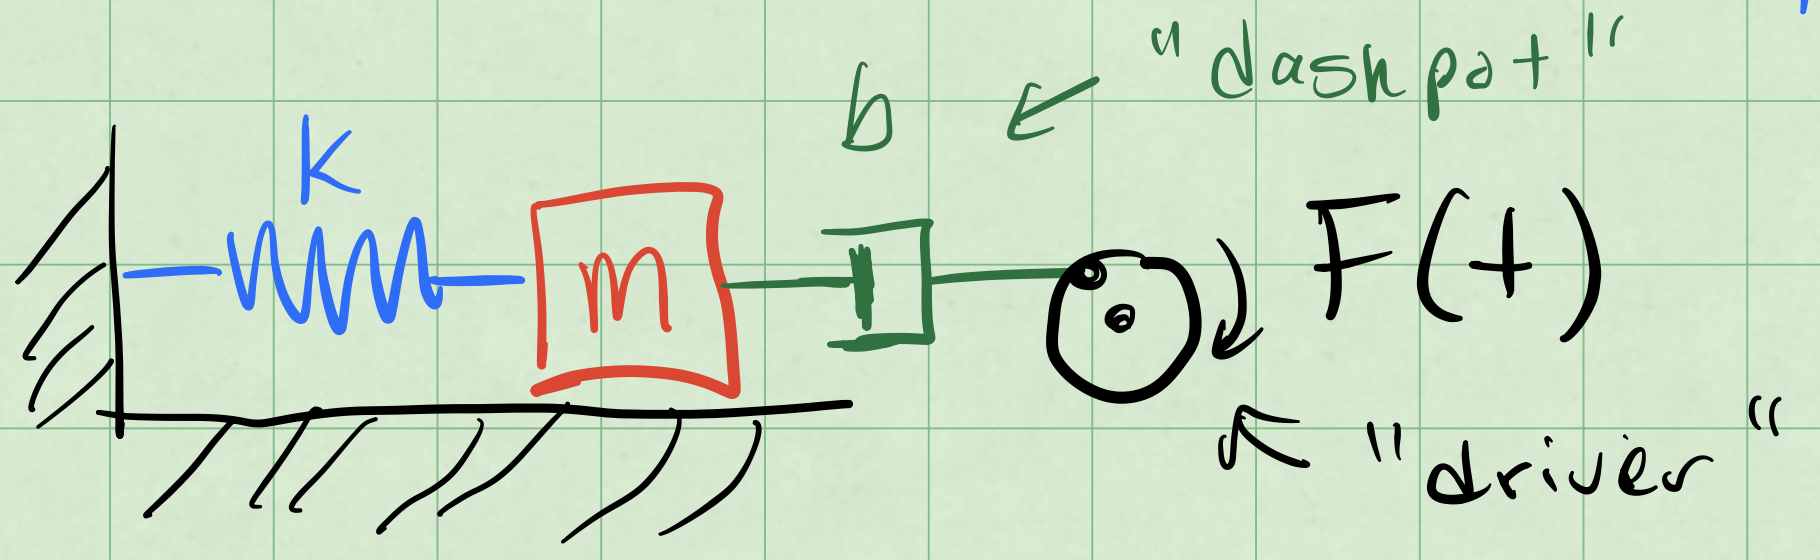
\includegraphics[keepaspectratio,alt={driven oscillator}]{/Users/caballero/repos/teaching/modern-classical-mechanics/images/notes/week9/driven_oscillator.png}}
\caption{driven oscillator}
\end{figure}

We write that differential equation as:

\[\ddot{x} + 2\beta \dot{x} + \omega_0^2 x = F(t)/m=f(t)\]

where \(\omega_0^2 = k/m\) and \(2\beta = b/m\). The function \(f(t)\)
is the driving force per unit mass.

\textbf{Note that this differential equation remains linear.}

Why? Because the ``operations'' on x(t) are linear.

    \subsection{Linearity of Differential
Equations}\label{linearity-of-differential-equations}

A linear differential equation has many nice properties. In particular,
the superposition of solutions and the uniqueness of solutions. So it is
worth knowing when you have one.

\textbf{Claim:} \(\dfrac{d}{dt}\) is a linear operator.

What is an operator? It is simply a function that takes a function as an
input and returns another function as an output. The derivative is a
function that takes a function and returns another function, namely the
slope of the tangent line to the original function everywhere it is
defined and differentiable.

Let's prove that \(\dfrac{d}{dt}\) is a linear operator.

Let \(x(t) = x_1(t) + x_2(t)\), where \(x_1(t)\) and \(x_2(t)\) are two
functions. Then

\[\dfrac{dx(t)}{dt} = \dfrac{d}{dt} \left(x_1(t) + x_2(t)\right) = \dfrac{dx_1(t)}{dt} + \dfrac{dx_2(t)}{dt}\]

We can distribute the derivative across the sum of the two functions.
Thus \(\dfrac{d}{dt}\) is a linear operator.

This also suggests that constants and other simple derivatives are
linear operators (e.g., \(\dfrac{d^2}{dt^2}\) and
\(\dfrac{d^3}{dt^3}\)). And because of the distributive property, any
linear sum of linear operators is also a linear operator (e.g.,
\(\dfrac{d^2}{dt^2} + \dfrac{d}{dt}\)).

    We can write the diffferential equation for the driven oscillator as

\[\dfrac{d^2x(t)}{dt^2} + 2\beta \dfrac{dx(t)}{dt} + \omega_0^2 x(t) = f(t).\]

We group the terms of the left hand side into a single operator,
\(\mathcal{D}\), so that

\[\mathcal{D} x(t) = \left(\dfrac{d^2}{dt^2} + 2\beta \dfrac{d}{dt} + \omega_0^2\right) x(t) = f(t)\]

The operator \(\mathcal{D}\) is a linear differential operator. This
compact notation expresses the linearity of the differential equation.

\[\mathcal{D} x(t) = f(t)\]

    \subsubsection{Effect of a Linear Operator on our
Solutions}\label{effect-of-a-linear-operator-on-our-solutions}

Because \(\mathcal{D}\) is a linear operator, we can distribute it. This
results in our finding a linear combination of solutions to the
differential equation. This is built up quite easily in three steps.

\begin{enumerate}
\def\labelenumi{\arabic{enumi}.}
\tightlist
\item
  We can allow the operator to act on a function scaled by a scalar
  constant \(a\):
\end{enumerate}

\[\mathcal{D} \left(a x(t)\right) = a \mathcal{D} x(t)\]

\begin{enumerate}
\def\labelenumi{\arabic{enumi}.}
\setcounter{enumi}{1}
\tightlist
\item
  We can allow the operator to act on a sum of functions:
\end{enumerate}

\[\mathcal{D} \left(x_1(t) + x_2(t)\right) = \mathcal{D} x_1(t) + \mathcal{D} x_2(t)\]

\begin{enumerate}
\def\labelenumi{\arabic{enumi}.}
\setcounter{enumi}{2}
\tightlist
\item
  We can allow the operator to act on a linear combination of functions:
\end{enumerate}

\[\mathcal{D} \left(a x_1(t) + b x_2(t)\right) = a \mathcal{D} x_1(t) + b \mathcal{D} x_2(t)\]

This is the superposition principle in action. But we have to be careful
when we apply it. For example, when,

\[\mathcal{D} x(t) = f(t)\]

we must first solve the homogeneous equation, \(\mathcal{D} x(t) = 0\).

    \subsection{Homogeneous and Particular
Solutions}\label{homogeneous-and-particular-solutions}

The damped driven oscillator is a linear differential equation. But that
means that any solution to the equation where the driving force is zero
is a solution to the equation where the driving force is non-zero. And,
thus must be added to the solution of the non-homogeneous equation.

Let's use the language of differential operators to express this. We
want to solve:

\[\mathcal{D} x(t) = f(t)\]

where \(\mathcal{D}\) is a linear differential operator. But any
solution to the homogeneous equation, \(\mathcal{D} x_h(t) = 0\), is a
solution to the non-homogeneous equation.

We use the notation \(x_h(t)\) to denote the solution to the homogeneous
equation.

So let's use the superposition principle to write the solution to the
non-homogeneous equation as a sum of two parts:

\[x(t) = x_h(t) + x_p(t)\]

where \(x_p(t)\) is a particular solution to the non-homogeneous
equation. We will get to the name of \(x_p(t)\) in a moment. Let's the
focus on the mathematical properties of the solution for a moment.

\[\mathcal{D} x(t) = \underbrace{\mathcal{D} x_h(t)}_0 + \mathcal{D} x_p(t) = f(t)\]

With the homogeneous solution, \(\mathcal{D} x_h(t) = 0\), we have

\[\mathcal{D} x_p(t) = f(t)\]

That is what defines the particular solution. In our case, that it is
specific to the driving force \(f(t)\) we have chosen.

\textbf{Summary:} When solving \(\mathcal{D} x(t) = f(t)\), the solution
is the sum of the homogeneous solution \(x_h(t)\) and a particular
solution \(x_p(t)\). We typically solve the homogeneous equation
\(\mathcal{D} x_h(t) = 0\) first.

The solutions \(x_h(t)\) satisfies the unknowns set by the initial
conditions. The particular solution \(x_p(t)\) is a solution to the
non-homogeneous equation \(\mathcal{D} x_p(t) = f(t)\), so it will not
depend on the initial conditions, how it is particular to the driving
force \(f(t)\).

    \subsection{Example: Sinusoidal Driving
Force}\label{example-sinusoidal-driving-force}

Let's consider a sinusoidal driving force. We will use the following
notation for the driving force:

\[f(t) = f_0 \cos(\omega t)\]

where \(f_0\) is the amplitude of the driving force and \(\omega\) is
the angular frequency of the driving force. \textbf{Note that \(\omega\)
is not necessarily the same as \(\omega_0\).}

So we can write the differential equation for the driven oscillator as

\[\mathcal{D} x(t) = f_0 \cos(\omega t)\]

where \(\mathcal{D}\) is the linear differential operator

\[\mathcal{D} = \dfrac{d^2}{dt^2} + 2\beta \dfrac{d}{dt} + \omega_0^2\]

Note that if instead \(f(t) = f_0 \sin(\omega t)\), then we would have

\[\mathcal{D} y(t) = f_0 \sin(\omega t)\]

where \(y(t)\) is the solution to the differential equation with a sine
driving force and \(\mathcal{D}\) is the same linear differential
operator. Writing both the \(x(t)\) of \(y(t)\) differential equations
out, we have

\[\ddot{x} + 2\beta \dot{x} + \omega_0^2 x = f_0 \cos(\omega t)\]
\[\ddot{y} + 2\beta \dot{y} + \omega_0^2 y = f_0 \sin(\omega t)\]

\subsubsection{Two Birds, One Stone}\label{two-birds-one-stone}

We can cleverly combine these two equations into a singlle differential
equation by using complex numbers.

\[z(t) = x(t) + i y(t).\]

We can similarly write \(f(t)\) as a complex sum:

\[f(t) = f_0 \cos(\omega t) + i f_0 \sin(\omega t) = f_0 e^{i \omega t}.\]

Now because of linearity, we can write the differential equation for
\(z(t)\) as

\[\mathcal{D} z(t) = f_0 e^{i \omega t}.\]

Written out, we have

\[\ddot{z} + 2\beta \dot{z} + \omega_0^2 z = f_0 e^{i \omega t}.\]

\subsubsection{Particular Solution}\label{particular-solution}

We note the particular solution depends on the driving force. We can try
one that follows the complex exponential form of the driving force.

\[z_p(t) = C e^{i \omega t}\]

where \(C\) is a complex constant. We can find \(C\) by substituting
\(z_p(t)\) into the differential equation.

\[\ddot{z}_p + 2\beta \dot{z}_p + \omega_0^2 z_p = f_0 e^{i \omega t}\]
\[\left(-\omega^2 + 2\beta i \omega + \omega_0^2\right) C e^{i \omega t} = f_0 e^{i \omega t}\]

We can cancel the \(e^{i \omega t}\) terms on both sides of the
equation, and we are left with

\[\left(-\omega^2 + 2\beta i \omega + \omega_0^2\right) C = f_0.\]

We can solve for \(C\):

\[C = \dfrac{f_0}{\omega_0^2 - \omega^2 + 2\beta i \omega}.\]

We found \(C\) and it is fully determined. But it is a complex number.
Ultimately, we want a real valued solution, but we remember that

\[Re(z(t)) = x(t) \qquad Im(z(t)) = y(t).\]

And we can write the coefficient \(C\) as a magnitude \(A\) and a phase
\(\delta\):

\[C = A e^{-i \delta}\]

\subsubsection{Writing the Complex
Amplitude}\label{writing-the-complex-amplitude}

Let's find that form of \(C\).

\[A^2 = CC^*\]
\[A^2 = \left(\dfrac{f_0}{\omega_0^2 - \omega^2 + 2\beta i \omega}\right) \left(\dfrac{f_0}{\omega_0^2 - \omega^2 - 2\beta i \omega}\right)\]
\[A^2 = \dfrac{f_0^2}{\left(\omega_0^2 - \omega^2\right)^2 + 4\beta^2 \omega^2}\]

So the amplitude of the particular solution is

\[A = \dfrac{f_0}{\sqrt{\left(\omega_0^2 - \omega^2\right)^2 + 4\beta^2 \omega^2}}.\]

We can find the phase by looking at \(C= A e^{-i \delta}\):

\[C = \dfrac{f_0}{\omega_0^2 - \omega^2 + 2\beta i \omega} = A e^{-i \delta}\]

\[f_0e^{i\delta} = A \left(\omega_0^2 - \omega^2 + 2\beta i \omega\right)\]

Note that both \(f_0\) and \(A\) are real numbers, so the complex phase
of \(\delta\) is determined by the complex number on the right side of
the equation.

That is, the phase of the \(e^{-i\delta}\) term and the phase of the
complex number \(\left(\omega_0^2 - \omega^2 + 2\beta i \omega\right)\)
are the same. So we can write ratio of their imaginary and real parts
as,

\[\tan(\delta) = \dfrac{2\beta \omega}{\omega_0^2 - \omega^2}\]

\[\delta = \arctan\left(\dfrac{2\beta \omega}{\omega_0^2 - \omega^2}\right)\]

Again, this number is fully determined without initial conditions.

\subsubsection{Back to the Particular
Solution}\label{back-to-the-particular-solution}

We proposed a solution \(z_p(t) = C e^{i \omega t}\), where \(C\) is a
complex constant. This became

\[z_p(t) = A e^{-i \delta} e^{i \omega t} = A e^{i(\omega t - \delta)}\]

where \(A\) is a real number and \(\delta\) is a real number. Note we
can write the particular solutions for both \(x(t)\) and \(y(t)\) as

\[x_p(t) = Re\left(z_p(t)\right) = A \cos(\omega t - \delta)\]
\[y_p(t) = Im\left(z_p(t)\right) = A \sin(\omega t - \delta)\]

\subsubsection{General Solution}\label{general-solution}

The proposed general solution was

\[x(t) = x_h(t) + x_p(t)\]

And for our sinusoidal driving force, we have found the particular
solution, so that we can write:

\[x(t) = x_h(t) + A \cos(\omega t - \delta)\]

where \(x_h(t)\) is the solution to the homogeneous equation,
\(\mathcal{D} x_h(t) = 0\).

We propose a solution form for \(x_h(t)\) that is a linear combination
of two exponential functions (as we did before):

\[x_h(t) = C_1 e^{\lambda_1 t} + C_2 e^{\lambda_2 t}.\]

These are solutions to the damped oscillator, and we refer to them as
the ``transient'' solutions. They are transient because they die out
over time due to damping.

For a weakly damped system, \(\beta^2 < \omega_0^2\), which is the case
that is most interesting to us, we can write the solution as,

\[x(t) = A \cos(\omega t - \delta) + A_{tr}e^{-\beta t} \cos(\omega_1 t - \delta_{tr})\]

where \(A_{tr}\) is the amplitude of the transient solution,
\(\omega_1 = \sqrt{\omega_0^2 - \beta^2}\) is the damped frequency (per
usual), and \(\delta_{tr}\) is the phase of the transient solution.

    \subsection{Resonance and Tuning}\label{resonance-and-tuning}

A curious thing about the long term behavior (after the transients die
out) is that we can observe large amplitudes at particular choices of
driving. Consider the long term (stady state) solution to the driven
damped harmonic oscillator:

\[x_{longterm}(t) = A \cos(\omega t - \delta)\]

where,

\[A^2 = \dfrac{f_0^2}{\left(\omega_0^2 - \omega^2\right)^2 + 4\beta^2 \omega^2}.\]

Let's allow \(\beta\) to be small so that \(4\beta^2 \omega^2\) is
small. If we focus on the denominator, we can see that the amplitude
will be small when \(\omega\) is far from \(\omega_0\). But if we choose
\(\omega\) to be close to \(\omega_0\), then the denominator will be
small, and the amplitude will be large.

The second result is a
\href{https://en.wikipedia.org/wiki/Resonance}{resonance} effect. The
system will resonate at a particular frequency, \(\omega_0\), and the
amplitude of the oscillations will be large. Below is a sketch of the
response of a driven damped harmonic oscillator to a sinusoidal driving
force. The amplitude of the oscillations is plotted as a function of the
driving frequency \(\omega\).

\begin{figure}
\centering
\pandocbounded{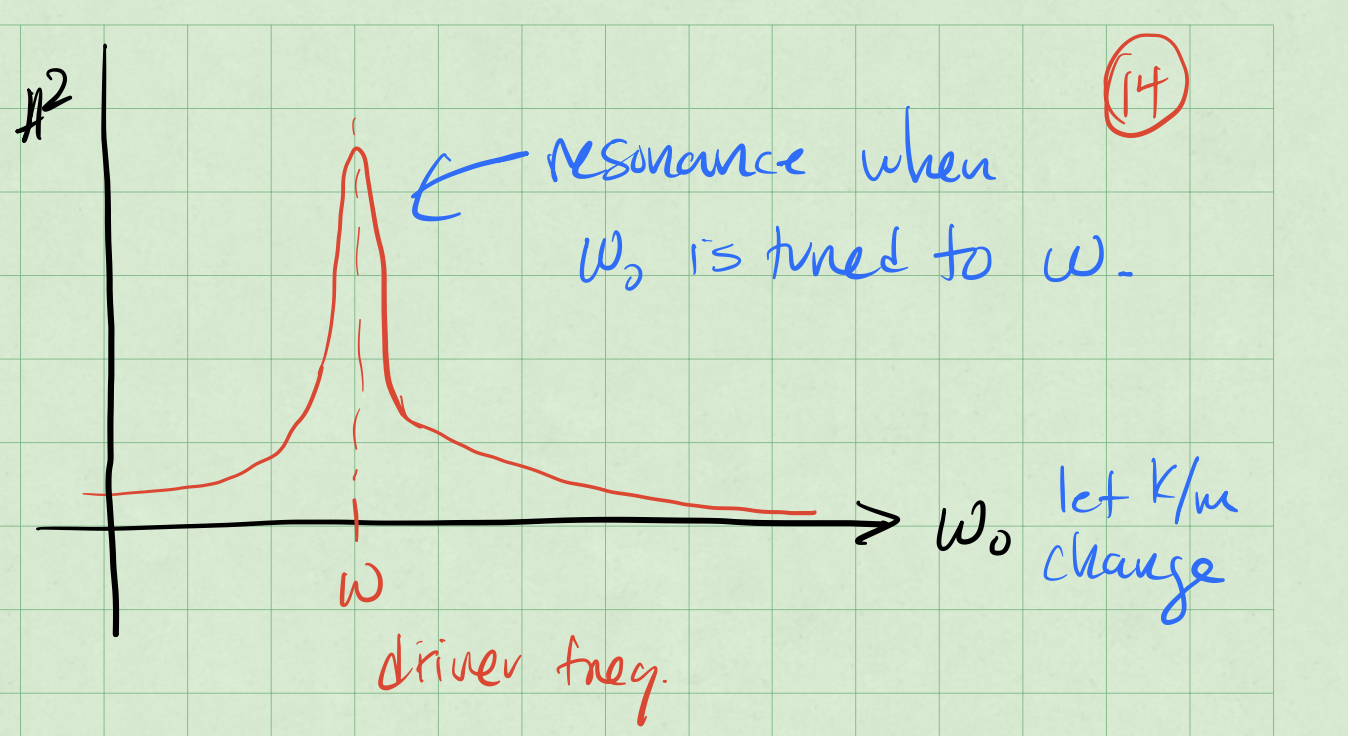
\includegraphics[keepaspectratio,alt={Resonance Sketch}]{/Users/caballero/repos/teaching/modern-classical-mechanics/images/notes/week9/resonance.png}}
\caption{Resonance Sketch}
\end{figure}

\subsubsection{Achieving Resonance}\label{achieving-resonance}

There's two ways that we can approach this. Let's focus on the
denominator of the amplitude equation:

\[\left(\omega_0^2 - \omega^2\right)^2 + 4\beta^2 \omega^2\]

When that denominator is small, the amplitude will be large. There's two
ways to make the denominator small.

\textbf{Case 1:} Tune the \(\omega_0\) (the natural frequency of the
system) to be close to \(\omega\) (the driving frequency). This is how a
car radio works. You change the resistance of the radio circuit to
change the natural frequency of the radio circuit. You can then tune the
radio to a particular station that is broadcasting at a particular
frequency. This gives an amplified signal,

When \(\omega_0 = \omega\), then the denominator is equal to
\(4\beta^2 \omega_0^2\). The amplitude is

\[A = \dfrac{f_0}{2\beta \omega_0}.\]

\textbf{Case 2:} Tune the driver (\(\omega\)) to be close to
\(\omega_0\).

Because we are adjusting the driver, we are seeking the driving
frequency that minizes the denominator. We can do this by setting the
derivative of the denominator with respect to \(\omega\) to zero.

\[\dfrac{d}{d\omega} \left(\left(\omega_0^2 - \omega^2\right)^2 + 4\beta^2 \omega^2\right) = 0\]

\[2\left(\omega_0^2 - \omega^2\right) \left(-2\omega\right) + 8\beta^2 \omega = 0\]

\[-4\omega_0^2 \omega + 4\omega^3 + 8\beta^2 \omega = 0\]

\[4\omega\left(\omega^2 - \omega_0^2 + 2\beta^2\right) = 0\]

\[\omega = 0 \qquad \text{or} \qquad \omega^2 - \omega_0^2 + 2\beta^2 = 0\]

Thie first solution is when there is no driver. But the second,
\(\omega_2\), is the frequency that minimizes the denominator. We can
write that as

\[\omega_2 = \sqrt{\omega_0^2 - 2\beta^2}\]

We can a strong response when \(\omega_0^2 \gg 2\beta^2\) or when
\(\omega_2 \approx \omega_0\).

    \begin{tcolorbox}[breakable, size=fbox, boxrule=1pt, pad at break*=1mm,colback=cellbackground, colframe=cellborder]
\prompt{In}{incolor}{ }{\boxspacing}
\begin{Verbatim}[commandchars=\\\{\}]

\end{Verbatim}
\end{tcolorbox}

    

    


    % Add a bibliography block to the postdoc
    
    
    
\end{document}
